\chapter{Zhodnocení testovací knihovny}\label{chap:review}

Vytvořená testovací knihovna splňuje požadavky a cíle, které na ní byly kladeny a které byly stanoveny v kapitole \ref{chap:cil}. Vyvstává zde ovšem otázka jak efektivní je toto řešení. V následujících sekcích je tedy vytvořené řešení zhodnocena na základě několika kritérií.

\section{Kategorie hodnocení}

Vytvořená testovací knihovna bude zhodnocena na základě těchto kategorií:

\begin{itemize}
    \item Flexibilita a možnosti použití knihovny
    \item Výkon virtualizované sítě
    \item Rychlost a efektivnost vytváření virtualizovaného prostředí
\end{itemize}

\noindent Všechny následující testy budou prováděny na počítači s těmito parametry:

\begin{itemize}
    \item Procesor - Intel Core i7-8850H
    \item Grafická karta - Nvidia Quadro P2000
    \item RAM - 16 GB
    \item Operační systém - Windows 10 Verze 21H2
\end{itemize}


\section{Flexibilita a možnosti použití knihovny}
Nová testovací knihovna lze využít pro jakékoliv testy, které vyžadují propojení zařízení, neboli kontejnerů, mezi sebou. Díky její implementaci je možné testy implementovat s libovolným počtem zařízení v různých topologiích.

Knihovna v aktuální podobě podporuje zařízení, které vychází z operačního systému Ubuntu. Tato podpora může být širší, protože závislost na systému Ubuntu je pouze na ty nástroje, které umožňují nastavení sítě na zařízení. Seznam kompatibilních systému ovšem zkoumám nebyl. Je zřejmé, že toto snižuje flexibilitu knihovny. Zároveň ovšem není náročné přidat další implementace pro jiné operační systémy. 

Prostor ke zlepšení je i v registraci testů. Jednotlivé testy jsou registrovány za pomoci výčtových typů, kde každý test je poté identifikován je číselnou hodnotou. Ideálním cílem je, aby všechny testové identifikátory byly definovány na jednom místě. V předchozí implementaci, která podporovala jazyky \csharp\,a\,\cpp\, bylo řešením tohoto problému jeden společný zdrojový soubor, díky čemuž byl problém vyřešen. S příchodem podpory jazyku Python to ale aktuálně není možné. Do budoucna je tedy vhodné investigovat způsob, kterým by byl tento problém vyřešen.

\section{Výkon virtualizované sítě}

Před započetím měření výkonu ve virtualizované síti vyvstává jednoduchá otázka - je možné navrhnout takový test, který s použitím testovací knihovny změří výkon virtualizované sítě? Odpověď na tuto otázku je pozitivní. 

Na měření výkonu sítě existuje jednoduchý nástroj iPerf3. Tento nástroj podporuje několik protokolů jako TCP nebo UDP a dovoluje nastavit různé parametry komunikace. Tento nástroj funguje na architektuře klient-server a je určen pro použití přes příkazovou řádku.

Zároveň ale existuje Python knihovna iPerf3, která zapouzdřuje tento nástroj pro použití v prostředí Python. To znamená, že ve spojení s Python implementací testovací knihovny jsme schopni vytvořit zařízení, které bude možné orchestrovat za pomoci testovací knihovny.

\subsection{Účastníci testu}

Součástí testu měření výkonu budou tito tři participanti:

\begin{itemize}
    \item Server
    \item Klient
    \item Zařízení pro vyplnění místa
\end{itemize}

Implementace těchto zařízení je velice podobná implementaci zařízení pro test s protokolem ModbusTCP v sekci \ref{sec:python_test_impl}. Návrh serveru a klient je totožný až na záměnu ModbusTCP serveru a klient na server a klient nástroje iPerf3. Pro nastavení parametrů testu je využito základních hodnot, které jsou nastaveny v nástroji iPerf. Jediná změněná hodnota byla délka testu, která byla nastavena na 60 sekund. Jednotlivé definice kontejnerů byly rozšířeny o balíček \inlinecode{libiperf-dev}, který obsahuje implementaci nástroje iPerf3. 

Nově ovšem přibylo zařízení pro vyplnění místa. Toto zařízení je aktivně připojené k testovací službě, jeho úkolem ovšem není provádět žádné testování. Zařízení na všechny požadavky o testování odpovídá kladně, i když sám žádné akce neprovádí. Jeho cílem je být výplní mezi serverem a klientem pro simulaci topologií a tím vzdálenosti mezi nimi. K tomuto úkolu by bylo možné použít jakékoliv zařízení, ovšem díky tomu, že zařízení bude aktivně připojeno k testovací službě se významně zrychlí orchestrace virtualizovaného prostředí a tím celého testování.


\subsection{Testované topologie}

K testování výkonu sítě byla zvolena topologie sériové linky. Primárním důvodem je, že všechny ostatní sítě se dají při komunikaci mezi serverem a klientem převést na sériovou linku. V případě kruhu zařízení komunikuje jednou cestou, dle nastavení statického směrování sítě. Následně v případě hvězdy je nejvzdálenější zařízení ve vzdálenosti maximálně dva. 

V následujících testech bude tedy 11 topologií, které budou pod označením \inlinecode{line-$x$.yaml}, kde číslo $x \in \{0,1,\dots, 10\}$ a značí počet zařízení vyplňujících zařízení mezi serverem a klientem.

\subsection{Výsledek testu a měření}

Výsledky z testů lze vidět na grafech níže. Jak lze vidět na grafu \ref{fig:graph_send_speed}, respektive \ref{fig:graph_receive_speed}, které znázorňují dosáhnutou rychlost přenosu dat v MB/s, tak při zvětšující se vzdáleností mezi klientem a serverem se snižuje rychlost přenosu. Nejnižší dosáhnutou rychlostí byla rychlost 990 MB/s. Tato rychlost je naprosto dostačující pro použití při testování. Na předem zmíněných grafech také můžeme vidět, že rychlost je symetrická. Daný procento počtu opakování přenosu se pohybuje mezi hodnotou 0.5 \% a 2.5 \%, což je akceptovatelné rozmezí pro využití knihovny.

\begin{figure}[htbp]
    \centering 
    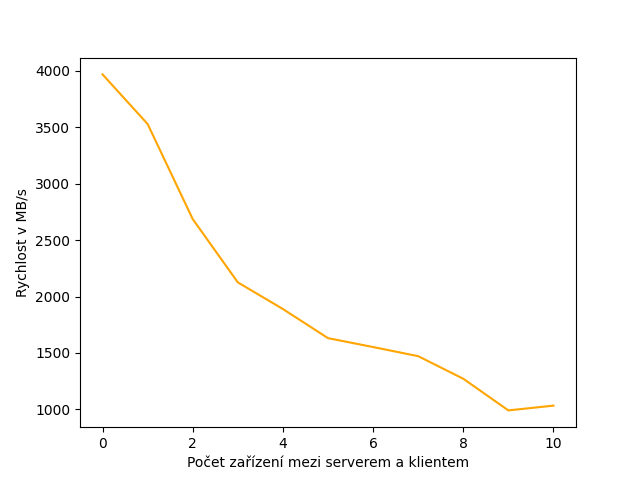
\includegraphics[width=0.8\textwidth]{assets/img/graphs/send_speed.png}
    \caption{Graf rychlosti odeslaných dat od klienta k serveru}
    \label{fig:graph_send_speed}
\end{figure}

\begin{figure}[htbp]
    \centering 
    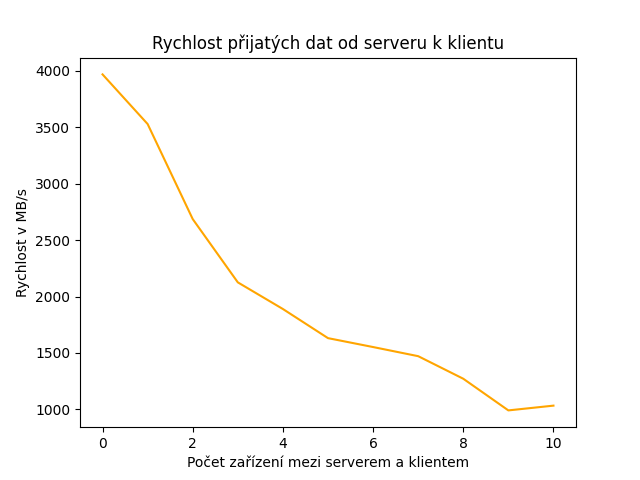
\includegraphics[width=0.8\textwidth]{assets/img/graphs/receive_speed.png}
    \caption{Graf rychlosti přijatých dat od serveru k klientu}
    \label{fig:graph_receive_speed}
\end{figure}

\begin{figure}[htbp]
    \centering 
    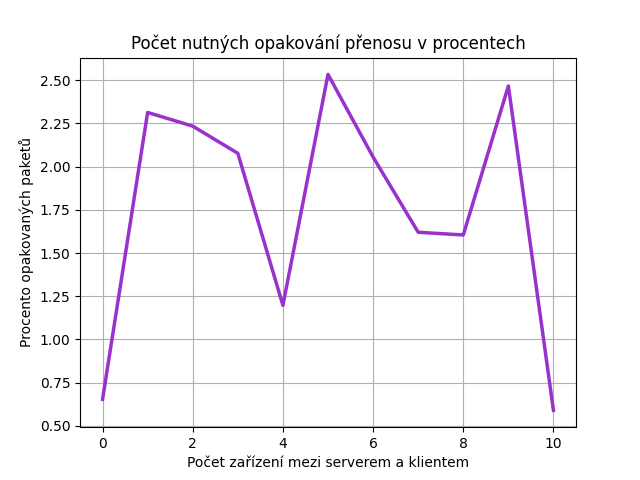
\includegraphics[width=0.8\textwidth]{assets/img/graphs/retransmissions.png}
    \caption{Graf procenta nutných opakování přenosu}
    \label{fig:graph_retransmissions}
\end{figure}


\section{Rychlost a efektivnost vytváření virtualizovaného prostředí}

K změření rychlosti vytváření virtualizované sítě byl využit stejný test, který byl definován v předchozí sekci. Při orchestraci tohoto testu bylo změřena doba potřebná doba k vytvoření virtualizovaného prostředí a doba potřebná k destrukci vytvořeného virtualizovaného prostředí. 

Naměřená dobu potřebnou k vytvoření virtualizovaného prostředí můžeme vidět na grafu \ref{fig:graph_create}. Jak je vidět, čas potřebný k vytvoření virtualizovaného prostředí roste lineárně. Je zde ale dobré přiblížit co se vlastně v tomto celém procesu děje. Tento test byl při vytváření prostředí schopen využít optimalizace, díky které je zabráněno opakovanému sestavování jednoho obrazu. Při každém vytváření virtualizovaného prostředí bylo nutné sestavit maximálně tři obrazy. Velikou část zabere vytváření sítě, respektive získávání informací o aktuálním stavu sítí ve virtualizovaném prostředí. Toto bylo vytvořeno s původní ideou, kdy na jednom stroji by mohlo běžet více instancí knihovny. Do budoucna by tedy bylo vhodné stav sítě ukládat a dotaz na stav sítě provádět pouze v případě chyby, kdy daný rozsah by byl zabrán. Zároveň zde může pomoct i optimalizace, kdy seznam již sestavených obrazů bude ukládán po celou dobu běhu testovací knihovny.

Čas potřebný k destrukci vytvořeného virtualizovaného prostředí lze vidět na obrázku \ref{fig:graph_remove}. Do tohoto času je zahrnuto odeslání zprávy od testovací služby o ukončení testování, které následně vede k ukončení daných zařízení, ukončení testovací služby a následně odstranění vytvořeného virtualizovaného prostředí. Z naměřených dat nelze vyvodit žádnou závislost na počtu vytvořených zařízení. Lze ovšem říci, že destrukce vytvořeného virtualizovaného prostředí v průměru trvala 19346.8 ms. 

Je ovšem vhodné podotknout, že čím více zařízení není ukončeno s pomocí testovací služby, tím víc narůstá čas potřebný k odstranění vytvořeného virtualizovaného prostředí. Tento nárůst vzniká primárně z časového limitu na nenásilné ukončení, na které software Docker čeká u každého kontejneru. Do budoucna je tedy vhodné investigovat jak odstranit tento časový limit, jelikož při použití GUI aplikace tento časový limit není přítomný. Při tomto testu bylo potřeba násilně ukončit pouze jedno zařízení.

\begin{figure}[htbp]
    \centering 
    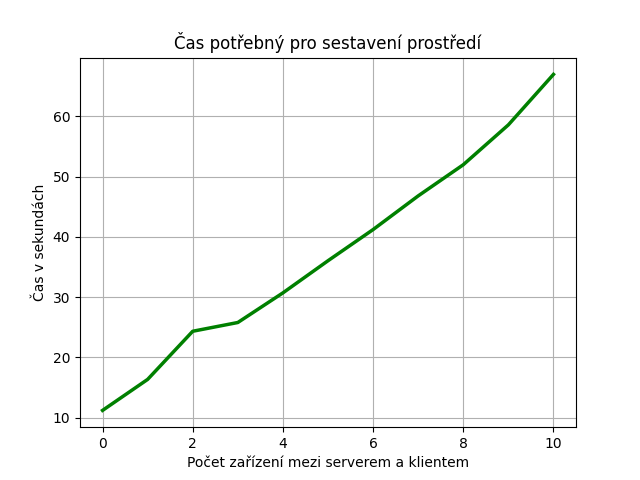
\includegraphics[width=0.8\textwidth]{assets/img/graphs/graph_start.png}
    \caption{Graf času potřebného k vytvoření virt. prostředí}
    \label{fig:graph_create}
\end{figure}



\begin{figure}[htbp]
    \centering 
    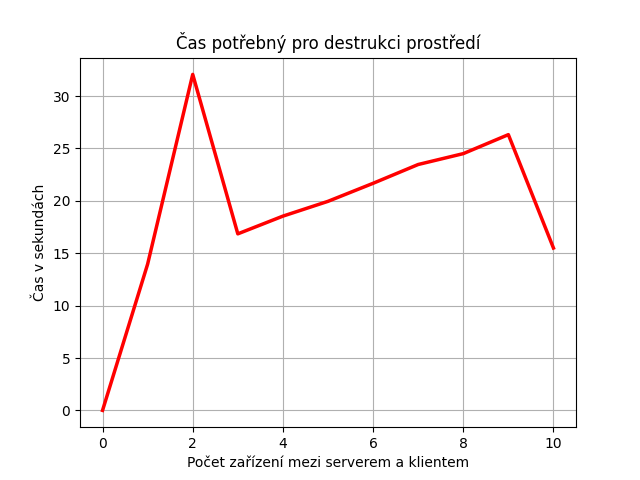
\includegraphics[width=0.8\textwidth]{assets/img/graphs/graph_remove.png}
    \caption{Graf času potřebného k odstranění virt. prostředí}
    \label{fig:graph_remove}
\end{figure}


\section{Shrnutí}

Dle naměřených hodnot vytvořená testovací knihovna výkonnostně a ergonomicky splňuje podmínka na ni kladené. Je zde ovšem stále prostor pro zlepšení. Z výkonnostního hlediska byly jasně definovány nedostatky ve vytváření a destrukci virtualizovaného prostředí, jejímž odstraněním se může zrychlit celý proces orchestrace virtualizovaného prostředí. Menší nedostatky byly nalezeny i v rámci použití samotné knihovny. Vyřešení těchto nedostatků ovšem nepřináší až tak vysoké benefity.


